\documentclass[11pt,oneside,openany,headings=optiontotoc,11pt,numbers=noenddot]{article}

\usepackage[a4paper]{geometry}
\usepackage[utf8]{inputenc}
\usepackage[T1]{fontenc}
\usepackage{lmodern}
\usepackage[ngerman]{babel}
\usepackage{ngerman}

\usepackage[onehalfspacing]{setspace}

\usepackage{fancyhdr}
\usepackage{fancybox}

\usepackage{rotating}
\usepackage{varwidth}

%Struktogramme
\usepackage[german,curves]{struktex}

\usepackage{pdflscape}
\usepackage{changepage}
\usepackage{graphicx}
\usepackage[bottom]{footmisc}
\usepackage{transparent}
\usepackage{graphbox}
\graphicspath{
	{Pics/PDFs/}
	{Pics/JPGs/}
	{Pics/PNGs/}
}
\usepackage{caption}
\usepackage{wrapfig}
\usepackage{marginnote}
\usepackage{tabularx}
\usepackage{dashrule}
\usepackage{soulutf8}
\usepackage{hhline}
%arydshln suppresses vertical lines in table
%\usepackage{arydshln}
\usepackage{multirow}
\usepackage{enumerate}
\usepackage[hidelinks]{hyperref}
\usepackage{listings}

\usepackage[table]{xcolor}
\usepackage{array}
\usepackage{enumitem,amssymb,amsmath}
\usepackage{interval}
\usepackage{cancel}
\usepackage{stmaryrd}
\usepackage{wasysym}
\usepackage{polynom}
\usepackage{diagbox}
\usepackage{dashrule}
\usepackage{framed}
\usepackage{mdframed}
\usepackage{karnaugh-map}
\usepackage{pdfpages}

\usepackage{blindtext}

\usepackage{eso-pic}

\usepackage{amssymb}
\usepackage{eurosym}

\usepackage[pages=some]{background}
\pagestyle{headings}
\renewcommand{\headrulewidth}{0.2pt}
\renewcommand{\footrulewidth}{0.2pt}
\newcommand*{\underdownarrow}[2]{\ensuremath{\underset{\overset{\Big\downarrow}{#2}}{#1}}}
\setlength{\fboxsep}{5pt}
\newcommand{\explainBelow}[3]{\underbrace{#1}_{\parbox{\widthof{#3}}{\footnotesize\raggedright #2}}}
\newcommand{\explainAbove}[3]{\overbrace{#1}^{\parbox{\widthof{#3}}{\footnotesize\raggedright #2}}}
\newcommand\footnoteref[1]{\protected@xdef\@thefnmark{\ref{#1}}\@footnotemark}


% Codestyle defined
\definecolor{codegreen}{rgb}{0,0.6,0}
\definecolor{codegray}{rgb}{0.5,0.5,0.5}
\definecolor{codepurple}{rgb}{0.58,0,0.82}
\definecolor{backcolour}{rgb}{0.95,0.95,0.92}
\definecolor{deepgreen}{rgb}{0,0.5,0}
\definecolor{darkblue}{rgb}{0,0,0.65}
\definecolor{mauve}{rgb}{0.40, 0.19,0.28}
\colorlet{exceptioncolour}{yellow!50!red}
\colorlet{commandcolour}{blue!60!black}
\colorlet{numpycolour}{blue!60!green}
\colorlet{specmethodcolour}{violet}

%Neue Spaltendefinition
\newcolumntype{L}[1]{>{\raggedright\let\newline\\\arraybackslash\hspace{0pt}}m{#1}}
\newcolumntype{M}{>{\centering\arraybackslash}X}
\newcommand{\cmnt}[1]{\ignorespaces}
%Textausrichtung ändern
\newcommand\tabrotate[1]{\rotatebox{90}{\raggedright#1\hspace{\tabcolsep}}}

%Intervall-Konfig
\intervalconfig {
	soft open fences
}

%Bash
\lstdefinestyle{BashInputStyle}{
	language=bash,
	basicstyle=\small\sffamily,
	backgroundcolor=\color{backcolour},
	columns=fullflexible,
	backgroundcolor=\color{backcolour},
	breaklines=true,
}
%Java
\lstdefinestyle{JavaInputStyle}{
	language=Java,
	backgroundcolor=\color{backcolour},
	aboveskip=1mm,
	belowskip=1mm,
	showstringspaces=false,
	columns=flexible,
	basicstyle={\footnotesize\ttfamily},
	numberstyle={\tiny},
	numbers=none,
	keywordstyle=\color{purple},,
	commentstyle=\color{deepgreen},
	stringstyle=\color{blue},
	emph={out},
	emphstyle=\color{darkblue},
	emph={[2]rand},
	emphstyle=[2]\color{specmethodcolour},
	breaklines=true,
	breakatwhitespace=true,
	tabsize=2,
}
%Python
\lstdefinestyle{PythonInputStyle}{
	language=Python,
	alsoletter={1234567890},
	aboveskip=1ex,
	basicstyle=\footnotesize,
	breaklines=true,
	breakatwhitespace= true,
	backgroundcolor=\color{backcolour},
	commentstyle=\color{red},
	otherkeywords={\ , \}, \{, \&,\|},
	emph={and,break,class,continue,def,yield,del,elif,else,%
		except,exec,finally,for,from,global,if,import,in,%
		lambda,not,or,pass,print,raise,return,try,while,assert},
	emphstyle=\color{exceptioncolour},
	emph={[2]True,False,None,min},
	emphstyle=[2]\color{specmethodcolour},
	emph={[3]object,type,isinstance,copy,deepcopy,zip,enumerate,reversed,list,len,dict,tuple,xrange,append,execfile,real,imag,reduce,str,repr},
	emphstyle=[3]\color{commandcolour},
	emph={[4]ode, fsolve, sqrt, exp, sin, cos, arccos, pi,  array, norm, solve, dot, arange, , isscalar, max, sum, flatten, shape, reshape, find, any, all, abs, plot, linspace, legend, quad, polyval,polyfit, hstack, concatenate,vstack,column_stack,empty,zeros,ones,rand,vander,grid,pcolor,eig,eigs,eigvals,svd,qr,tan,det,logspace,roll,mean,cumsum,cumprod,diff,vectorize,lstsq,cla,eye,xlabel,ylabel,squeeze},
	emphstyle=[4]\color{numpycolour},
	emph={[5]__init__,__add__,__mul__,__div__,__sub__,__call__,__getitem__,__setitem__,__eq__,__ne__,__nonzero__,__rmul__,__radd__,__repr__,__str__,__get__,__truediv__,__pow__,__name__,__future__,__all__},
	emphstyle=[5]\color{specmethodcolour},
	emph={[6]assert,range,yield},
	emphstyle=[6]\color{specmethodcolour}\bfseries,
	emph={[7]Exception,NameError,IndexError,SyntaxError,TypeError,ValueError,OverflowError,ZeroDivisionError,KeyboardInterrupt},
	emphstyle=[7]\color{specmethodcolour}\bfseries,
	emph={[8]taster,send,sendMail,capture,check,noMsg,go,move,switch,humTem,ventilate,buzz},
	emphstyle=[8]\color{blue},
	keywordstyle=\color{blue}\bfseries,
	rulecolor=\color{black!40},
	showstringspaces=false,
	stringstyle=\color{deepgreen}
}

\lstset{literate=%
	{Ö}{{\"O}}1
	{Ä}{{\"A}}1
	{Ü}{{\"U}}1
	{ß}{{\ss}}1
	{ü}{{\"u}}1
	{ä}{{\"a}}1
	{ö}{{\"o}}1
}

% Neue Klassenarbeits-Umgebung
\newenvironment{worksheet}[3]
% Begin-Bereich
{
	\newpage
	\sffamily
	\setcounter{page}{1}
	\ClearShipoutPicture
	\AddToShipoutPicture{
		\put(55,761){{
				\mbox{\parbox{385\unitlength}{\tiny \color{codegray}BBS I Mainz, #1 \newline #2
						\newline #3
					}
				}
			}
		}
		\put(455,761){{
				\mbox{\hspace{0.3cm}
\includegraphics[width=0.2\textwidth]{../../logo.pdf}}
			}
		}
	}
}
% End-Bereich
{
	\clearpage
	\ClearShipoutPicture
}

\setlength{\columnsep}{3em}
\setlength{\columnseprule}{0.5pt}

\geometry{left=1.50cm,right=1.50cm,top=2.50cm,bottom=1.00cm,includeheadfoot}
\pagenumbering{gobble}
\pagestyle{empty}

\begin{document}
	\begin{worksheet}{Berufliches Gymnasium}{Klassenstufe 12 - Informationsverarbeitung}{Lernabschnitt 1: Netzwerke - Netzwerk-Kommunikation - OSI-Schichtenmodell}
		\setcounter{section}{1}
		\setcounter{subsection}{3}
		\subsection{OSI-Schichtenmodell}
		Bei der Kommunikation in der IT unterscheidet man zwischen \textbf{geschlossenen} und \textbf{offenen} Kommunikationssystemen.
		\begin{itemize}[label=$\circ$]
			\item Unter einem \textbf{geschlossenen} System verstehen wir ein von Hersteller abhängiges System, das individuelle firmenbezogene Protokolle, Zeichensätze und Übertragungssequenzen nutzt, welche in der Regel nicht veröffentlicht werden. Das bedeutet, dass eine Kommunikation mit Geräten von Fremdfirmen nicht  möglich ist.
			\item In einem \textbf{offenen} System werden Richtlinien eingehalten, welche anderen Herstellern die Möglichkeit geben, kompatible Geräte zu bauen oder auch entsprechende Anpassungen an den Schnittstellen zu schaffen, so dass eine Verwendung von Geräten anderer Hersteller möglich ist.\\
			Um diese Richtlinien bzw. Standards zu vereinheitlichen, wurde das \grqq{}\textbf{Referenzmodell für die Kommunikation offener Systeme}\grqq{}\footnote{Auch als \textit{ISO-Modell}, \textit{OSI-Modell} (\textbf{OSI}: \textbf{O}pen \textbf{S}ystem \textbf{I}nterconnection) oder auch \textit{7-Schichten-Modell} bezeichnet.} geschaffen. 
		\end{itemize}
		Das Referenzmodell wird auch als  Die einzelnen Schichten werden auch als \textbf{Ebenen} oder \textbf{Layer} bezeichnet. Jeder Schicht kommt eine klar definierte Aufgabe bei der Kommunikation zu.\\
		Die Schichten 1 bis 4 erden als \textbf{transportorientierte Schichten} bezeichnet, währen die Schichten 5 bis 7 als \textbf{anwendungsorientierte Schichten} verstanden werden. Bildlich gesehen, kann man sich die Schichten als Stapel vorstellen, so dass man das gesamte Konstrukt auch häufig als \textbf{Protokoll-Stapel} bezeichnet.
		\subsubsection{Ablauf der Kommunikation}
		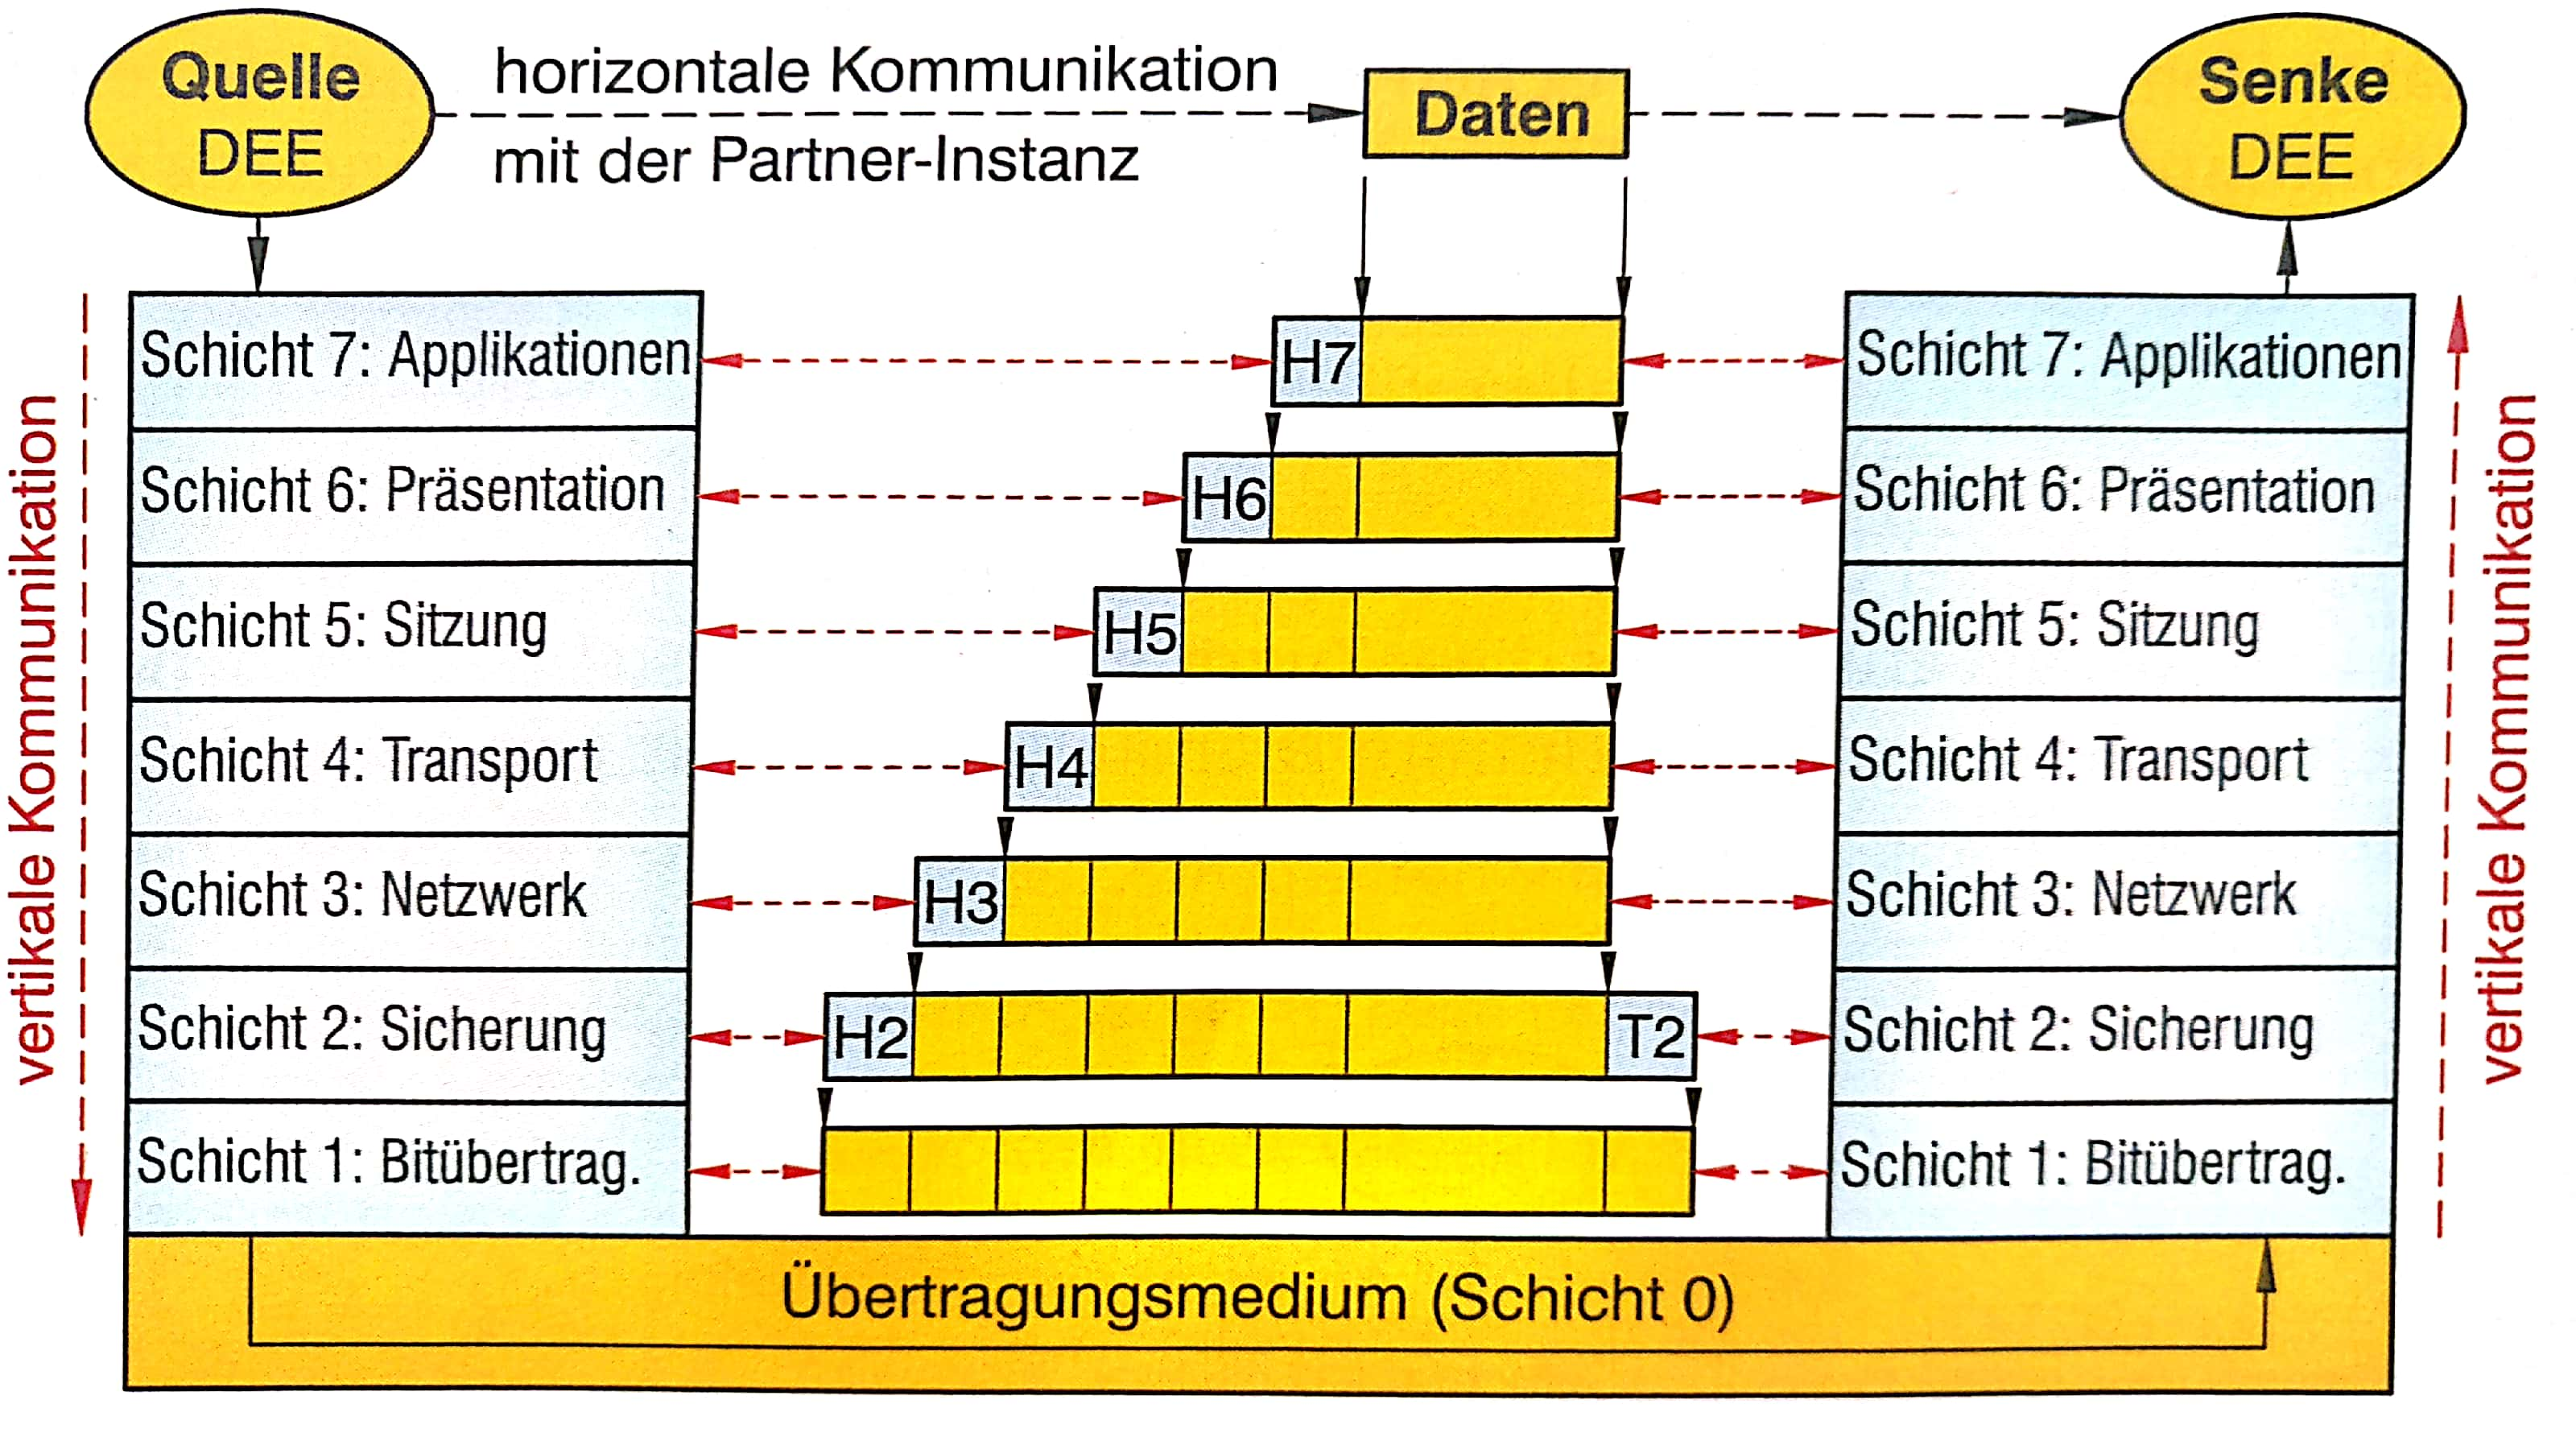
\includegraphics[width=\textwidth]{../99_Bilder/042_QueSen.jpg}\\
		\tiny{\texttt{Quelle: Vernetzte IT-Systeme, Basiswissen IT-Berufe von Frisch, Hölzel, Lintermann, Schaefer; S. 25.}}\normalsize\\
		\par\noindent
		Den genauen Ablauf der Kommunikation zwischen \textbf{Quelle} (Sender) und der \textbf{Senke} (Empfänger) kann man sich wie folgt vorstellen:\\
		Das zu übertragende Datenpaket wird auf der Senderseite von der \textbf{Datenendeinrichtung} (DEE) erzeugt und durchläuft anschließend die Schichten 7 bis 1 des OSI-Modells.
		\begin{framed}
			\noindent
			\textbf{\underline{Vertikale Kommunikation}}\\Der Weg des Datenpakets durch die einzelnen Schichten des OSI-Modells wird auch als \textbf{vertakel Kommunikation} bezeichnet.
		\end{framed}
		\noindent
		Innerhalb jeder Schicht wird dem Übergebenen Nutzdatenpaket (Payload) eigene Protokollinformationen hinzu. Hierbei unterscheidet man zwischen den am Anfang befindlichen Informationen, dem sogenannten \textbf{Header}\footnote{Protokollkopf, -vorspann.}, und den am Ende befindlichen Informationen, \textbf{Trailer}\footnote{Protokollnachspann.}.\\
		Jede Schicht behandelt die zuvor hinzugefügten Header bzw. Trailer als Nutzdaten und werden von der aktuell behandelnden Schicht in keinster Weise interpretiert oder verändert.\\
		Die Schicht 1: Bitübertragung wandelt das gesamte Nutzdatenpaket mit allen Protokollinformationen in technisch übertragbare Signale um und transportiert diese dann über das genutzte Übertragungsmedium.\\
		\par\noindent
		Auf Empfängerseite durchläuft das Paket die Schichten 1 bis 7.Sind die Signale beim Empfänger angelangt, werden diese zunächst von Schicht 1 in Nutzdaten (Paket) umgewandelt. Anschließend werden die zuvor hinzugefügten Protokollinformationen nacheinander wieder entfernt. Dieser Vorgang wird Schichtweise durchgeführt, so dass die Protokollinformationen von Schicht 3 nur von Schicht 3 des Empfängers entfernt und verarbeitet werden können.
		\begin{framed}
			\noindent
			\textbf{\underline{Horizontale Kommunikation}}\\
			Jede Schicht der Senderseite kann nur mit der entsprechenden Schicht auf der Empfängerseite korrespondieren (\textbf{horizontale Kommunikation}).
		\end{framed}
		\noindent
		Die Kommunikation auf horizontaler Ebene ist rein logisch. Lediglich die Schicht 1 steht in einer physikalischen Verbindung.
		\subsubsection{Ablauf der Datenübertragung}
		Angenommen der Anwender an \textbf{System A} möchte mit einem Anwendung Daten an ein anderes \textbf{System B} sende, werden diese Daten zunächst von der Anwendung an die entsprechende \textbf{Anwendungsschicht} übergeben.\\
		Auf der Anwendungsschicht werden relevante Steuerdaten vor die Daten (als Header) angefügt. Diese Nutzdaten (Header mit Daten) werden an die \textbf{Darstellungsschicht} übergeben. Auch diese erweitert den Header um für die Partnerschicht von System B relevante Daten.\\
		Das vergrößerte Nutzdatenpaket (Header und die Daten) wird an die nächste Schicht, die \textbf{Sitzungsschicht} übergeben. Diese erweitert den Header erneut und reicht das Gesamtpaket an die \textbf{Transportschicht} weiter.\\
		Die Transportschicht teilt das Datenpaket in kleinere Teile (\textbf{Datensegmente}) auf, sodass diese leichter zu verarbeiten sind. Jedem Datensegment wird eine eindeutige Nummer zugeteilt, so dass der Empfänger erkennen kann, in welche Reihenfolge die Segmente gehören.\\
		Nachdem das Datenpaket in Datensegmente unterteilt wurde, kapselt die \textbf{Vermittlungsschicht} die einzelnen Segmente in \textit{Datenpakete}. Diese werden anschließend noch um die Ziel- und die Quellnetzadresse (standardmäßig die IP-Adresse) erweitert.\\
		Jedes Datenpaket wird an die \textbf{Sicherungsschicht} übergeben und diese generiert daraus \textit{Datenframes}. Diesem wird dann die physikalische Quell- und Zieladresse (die MAC-Adresse) hinzugefügt.\\
		Sind die Datenframes erzeugt, übernimmt die \textbf{Bitübertragungsschicht} die Aufgabe, diese in ein Muster aus 0en und 1en zu überführen. Dies ist notwendig, da nur diese kodierten Daten über das Medium übertragen werden können.\\
		\par\noindent
		Sind die Bits übertragen, empfangen und von der \textit{Bitübertragungsschicht} umgewandelt worden, gibt diese die Datenframes an die nächst höher liegende Schicht weiter. Dort werden die Header bzw. Trailer entfernt, die von der gleichen Schicht in System A hinzugefügt wurden.\\
		Dies geschicht, bis alle Header bzw. Trailer entfernt und die Daten auf der Anwendungsschicht angelangt sind, wird der letzte Header, nämlich der der Anwendungsschicht entfernt und die Rohdaten werden in der Anwendung von System B angezeigt.
		\begin{framed}
			\noindent
			Das übermittelte Datenpaket durchläuft auf Empfängerseite in umgekehrter Reihenfolge die gleichen Schichten. Die Protokolle jeder Schicht entfernen die hinzugefügten Informationen und reichen die übrigen Daten an die nächste Schicht weiter.
		\end{framed}
		\subsubsection{Services und Schnittstellen}
		Jede Schicht des OSI-Modells bietet bestimmte Dienstleistungen, auch \textbf{Services}, welche von der jeweils höher liegenden Schicht genutzt werden kann. Um die eigenen Dienste zur Verfügung zu stellen, greift die jeweilige Schicht auf die Dienste der darunterliegenden Schicht zu.\\
		\begin{minipage}{0.58\textwidth}
			Um diese Zugriffe zu ermöglichen, wurden Schnittstellen zwischen den einzelnen Schichten definiert. An diesen können auf spezielle Dienste der entsprechenden Schicht zugegriffen werden. Diese Zugriffspunkte werden auch \textbf{Service Access Points} (SAP) genannt.
		\end{minipage}
		\hfill
		\begin{minipage}{0.4\textwidth}
			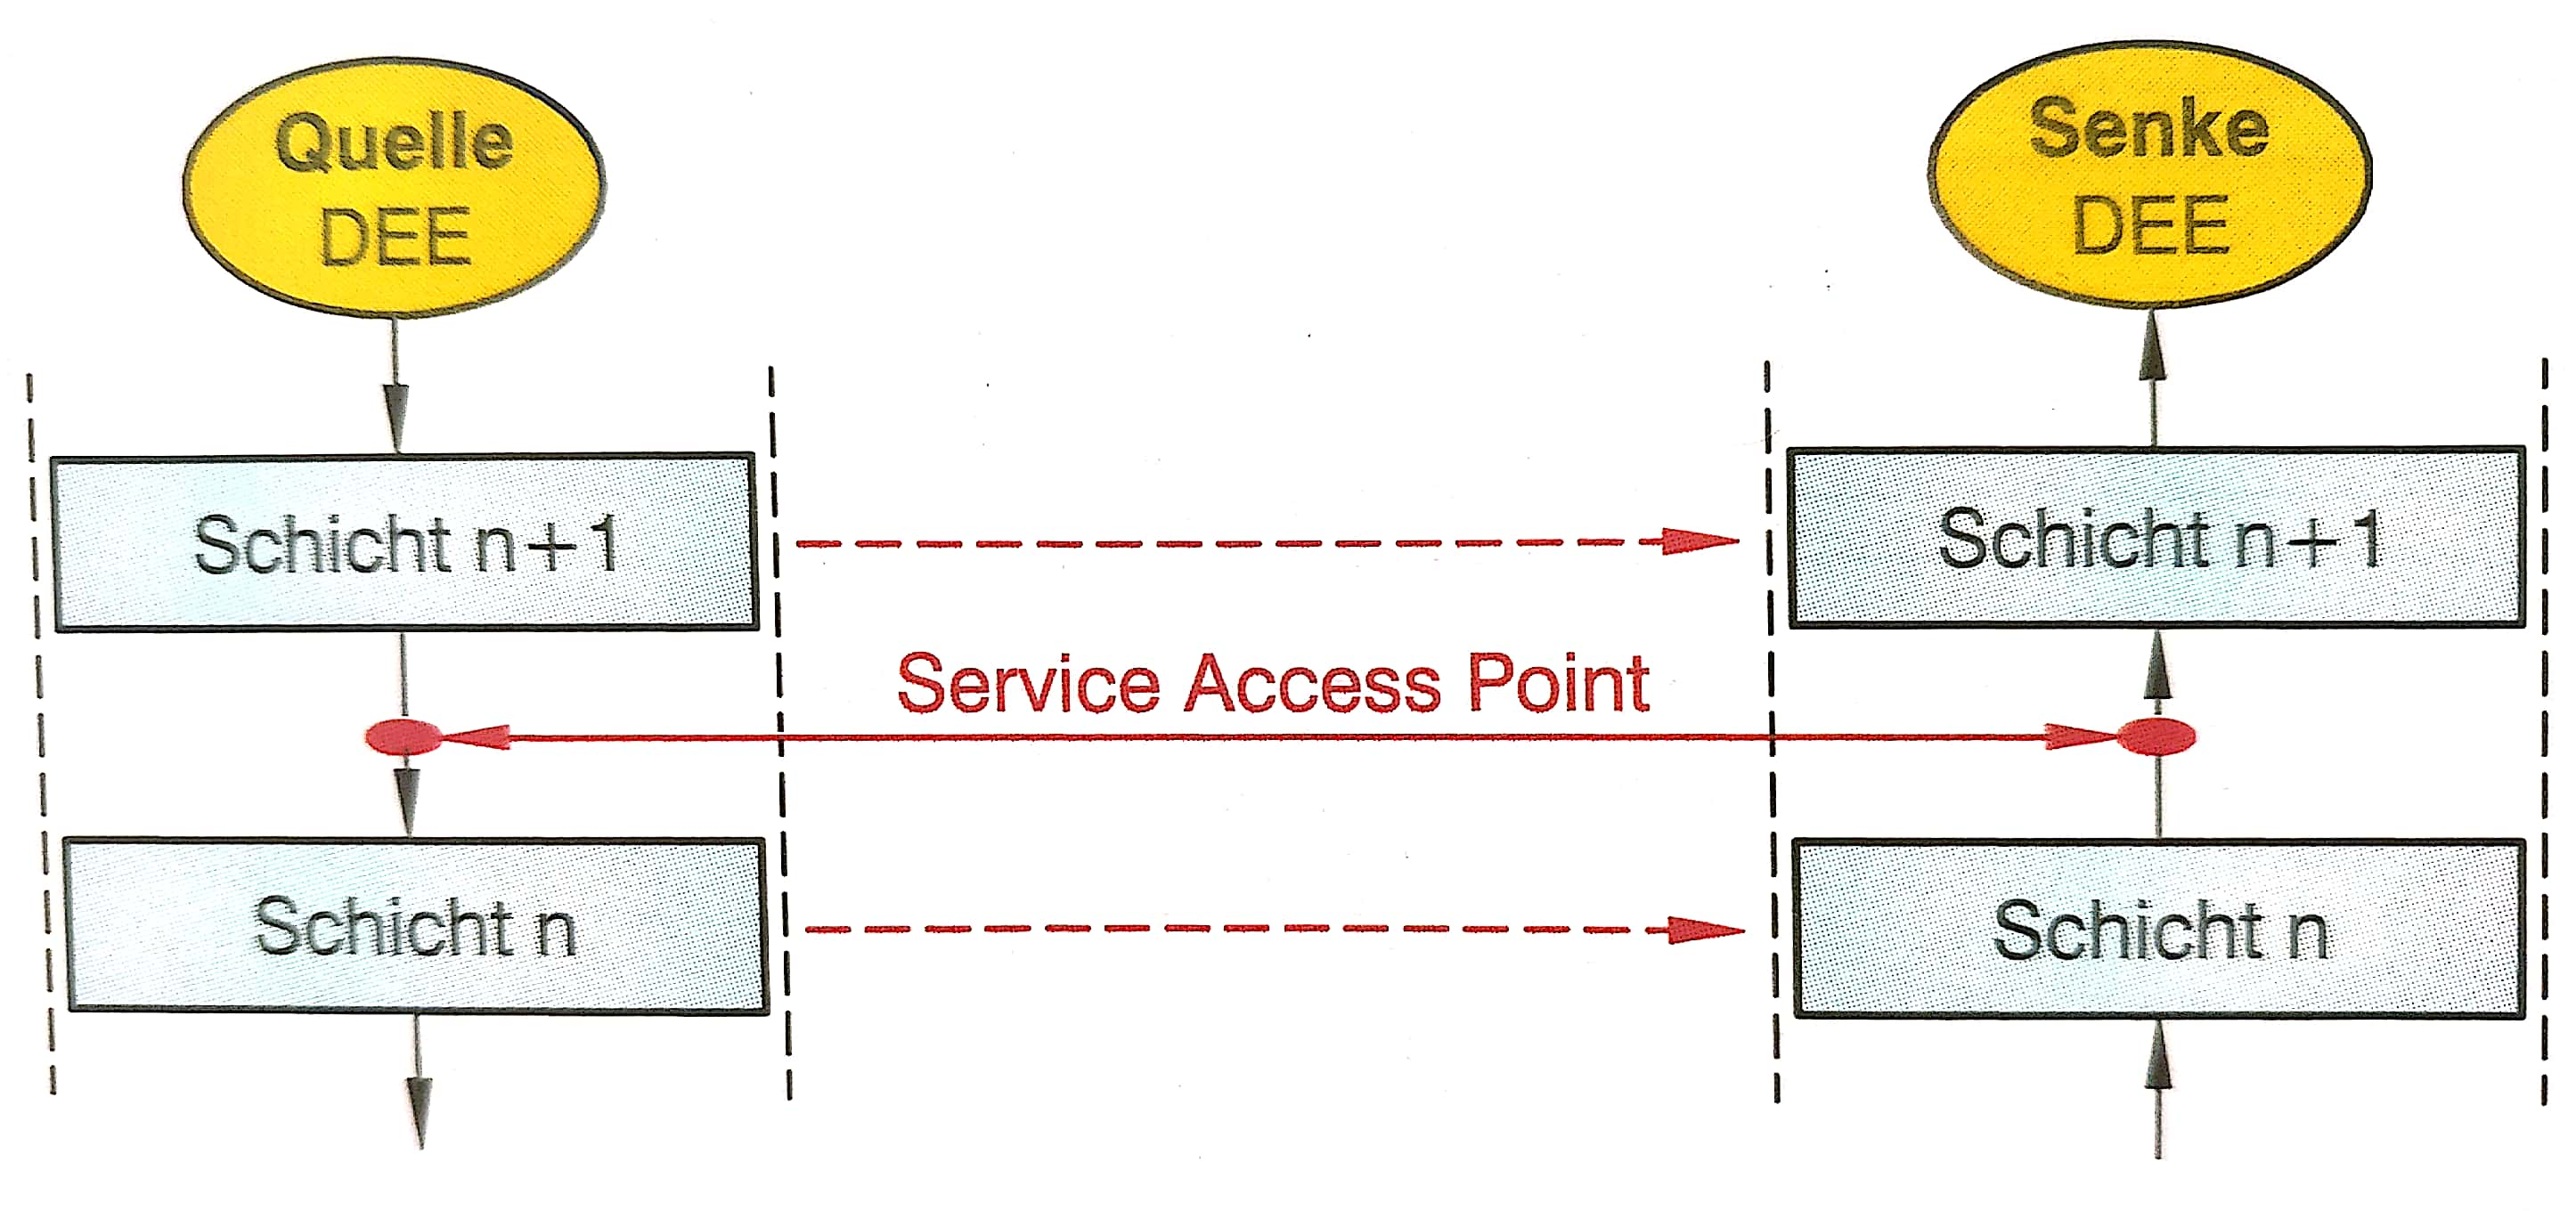
\includegraphics[width=0.85\textwidth]{../99_Bilder/042_SAP.jpg}\\
			\tiny{\texttt{Quelle: Vernetzte IT-Systeme, Basiswissen IT-Berufe von Frisch, Hölzel, Lintermann, Schaefer; S. 26.}}\normalsize\\
		\end{minipage}
		Befinden sich Quelle und Senke bei der Kommunikation nicht in direkter Verbindung, läuft diese über ein zwischengeschaltetes Übertragungsgerät. Häufig nennt man diese auch \textbf{Datenübertragungseinrichtung} (DÜE) bezeichnet.\\
		\par\noindent
		\begin{center}
			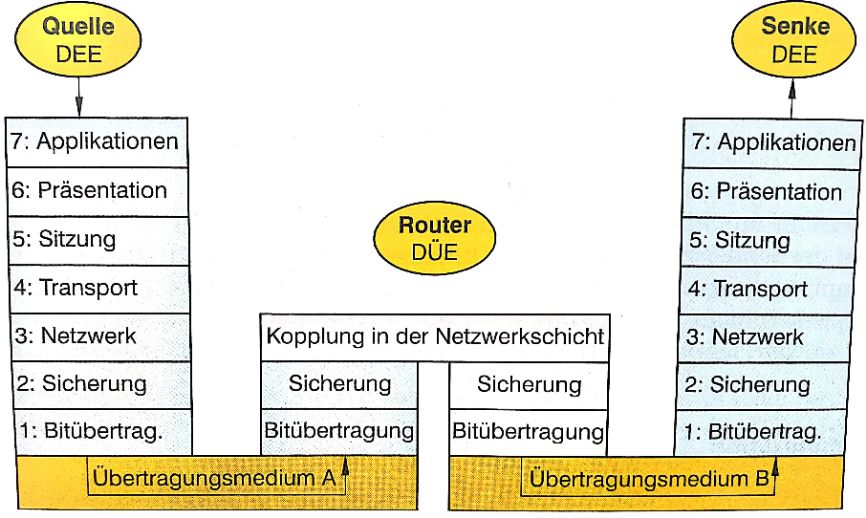
\includegraphics[width=0.9\textwidth]{../99_Bilder/042_Rou.jpg}\\
			\tiny{\texttt{Quelle: Vernetzte IT-Systeme, Basiswissen IT-Berufe von Frisch, Hölzel, Lintermann, Schaefer; S. 26.}}\normalsize\\
		\end{center}
		Wie in der Grafik erkennbar, müssen in einer \textbf{DÜE} nicht alle Schichten realisiert sein.
		\subsubsection{Funktionen der einzelnen Schichten}
		In der nachfolgenden Tabelle werden die Bezeichnungen sowie die Aufgaben der einzelnen Schichten (Layer) dargestellt:\\
		\par\noindent
		\renewcommand{\arraystretch}{1.5}
		\begin{tabularx}{\textwidth}{|c|c|X|}
			\hline
			\rowcolor{gray!10} \textbf{Schicht} & \textbf{Bezeichnung} & \textbf{Hauptaufgabe der Schicht}\\
			\hline
			7 & Applikation & Anfragen werden von Anwendungen entgegengenommen und ausgeführt.\\
			\hline
			6 & Präsentation & Wandelt Daten der Applikationsschicht in geeignete Formate um.\\
			\hline
			5 & Sitzung & Organisiert die Sitzung / Verbindung zwischen zwei Partnern.\\
			\hline
			4 & Transport & Handelt als Brücke zwischen anwendungs- und transportorientierten Schichten. Stellt sicher, dass übermittelte Daten sicher beim Partner ankommen.\\
			\hline
			3 & Netzwerk & Organisiert die Kommunikation zwischen den Endgeräten. Fügt dem Datenpaket erstmals eine logische Adresse zu.\\
			\hline
			2 & Sicherung & Gewährleistet eine zuverlässige und vollständige Datenübertragung. Die Schicht hat die Möglichkeit Fehler zu erkennen und diese zu beheben.\\
			\hline
			1 & Bitübertragung & Wandelt das Nutzdatenpaket in übertragbare Signale um und definiert somit die elektrische, mechanische und funktionale Schnittstelle zum Übertragungsmedium.\\
			\hline
		\end{tabularx}
	\end{worksheet}
\end{document}